\documentclass[11pt,conference]{IEEEtran}

\ifCLASSINFOpdf
   \usepackage[pdftex]{graphicx}
  % declare the path(s) where your graphic files are
   \graphicspath{{../pdf/}{../jpeg/}}
  % and their extensions so you won't have to specify these with
  % every instance of \includegraphics
   \DeclareGraphicsExtensions{.pdf,.jpeg,.png}
\else
  % or other class option (dvipsone, dvipdf, if not using dvips). graphicx
  % will default to the driver specified in the system graphics.cfg if no
  % driver is specified.
  \usepackage[dvips]{graphicx}
  % declare the path(s) where your graphic files are
  \graphicspath{{../eps/}}
  % and their extensions so you won't have to specify these with
  % every instance of \includegraphics
  \DeclareGraphicsExtensions{.eps}
\fi


\usepackage[utf8x]{inputenc}
\usepackage[T1]{fontenc}
\usepackage{lmodern}
\usepackage{booktabs}
\usepackage{multirow}
\usepackage{algorithmic}
\usepackage[Algoritmo]{algorithm}
\usepackage[spanish,USenglish]{babel}
\usepackage[colorlinks=true,linkcolor=black,urlcolor=black,citecolor=black, urlcolor=black, filecolor=black bookmarks=false]{hyperref}
\usepackage{subfigure}
\usepackage{array}
\usepackage{color}
\usepackage{graphicx}
\usepackage{epsfig}
\usepackage{multirow}
\usepackage{colortbl}
\usepackage[table]{xcolor}

\addto\captionsspanish{
 \def\tablename{Tabla}}


\begin{document}

\pagestyle{empty}  

\selectlanguage{spanish}

\title{Informe trabajo práctico número uno - Aprendizaje Automático}

\author{\IEEEauthorblockN{Omar Ernesto Cabrera Rosero}
\IEEEauthorblockA{Universidad de Buenos Aires\\
%Buenos Aires, Argentina\\
Email: omarcabrera@udenar.edu.co}
\and
\IEEEauthorblockN{Jimmy Mateo Guerrero Restrepo}
\IEEEauthorblockA{Universidad de Buenos Aires\\
%Buenos Aires, Argentina\\
Email: jimaguere@gmail.com}
}

\maketitle

%\selectlanguage{USenglish}
\begin{abstract}

En este trabajo práctico se analizan las particularidades de la utilización de
algoritmos para la generación de árboles de decisión, para la aplicación se utilizó un conjunto de datos
de las pruebas de estado de calidad de la educación
superior Saber Pro en Colombia, según el decreto 3963 del 14 de octubre de 2009 \cite{men2009},
a estudiantes próximos a culminar los programas académicos de pregrado que ofrecen las instituciones
de educación superior.
\end{abstract}
 
\selectlanguage{spanish}


\begin{IEEEkeywords}
Árboles de decisión, J48, Saber Pro, sobreajuste
\end{IEEEkeywords}

\thispagestyle{empty} 

\IEEEpeerreviewmaketitle

\section{Introducción}

El objetivo del presente informe es presentar los resultados del análisis del
comportamiento del algoritmo de aprendizaje de árboles de decisión J48 en función del
Confidence Factor (CF) y evaluar aspectos como el sobreajuste y su robustez ante
variaciones en el conjunto de datos. La variaciones en el conjunto de datos que fueron 
tenidas en cuenta fueron: datos faltantes, la tolerancia al ruido y la
discretización de atributos numéricos.

El conjunto de datos utilizado es de las pruebas de estado Saber Pro 2012-1 en Colombia,
uno de los objetivos del examen de estado de calidad de la educación superior Saber
Pro, según el decreto 3963 del 14 de octubre de 2009, Ministerio de Educación
Nacional \cite{men2009}, es comprobar el grado de desarrollo de competencias de los
estudiantes próximos a culminar los programas académicos de pregrado que ofrecen
las instituciones de educación superior. El examen está compuesto por pruebas que
evalúan competencias genéricas y específicas. De acuerdo a los lineamientos Saber
Pro del Instituto colombiano para el Fomento de la Educación Superior \cite{icfes2011},
todos los estudiantes deben presentar los módulos de competencias genéricas sin
importar el programa de formación que cursen, que incluye competencias de
razonamiento cuantitativo, lectura crítica, escritura e inglés.

En la competencia de razonamiento cuantitativo se evalúan los desempeños
relacionados con uso de lenguaje cuantitativo y solución de problemas \cite{icfes2012a}.
En la competencia de lectura crítica se evalúan los desempeños asociados a lectura,
pensamiento crítico y entendimiento interpersonal \cite{icfes2012a}. En escritura se
evalúa la competencia para comunicar ideas por escrito referidas a un tema dado
\cite{icfes2011} \cite{icfes2012a}. En inglés se evalúa la competencia del estudiante para
comunicarse efectivamente en inglés.

El conjunto de datos pertenece a los datos de las pruebas Saber Pro 2012-1, la cual cuenta con
94 variables y 97.068 registros, a este conjunto de datos se le realizó un tratamiento de transformación
de variables para reducir la dimesión, con esto se obtuvo un nuevo conjunto de datos con 31 variables y
96.775 registros. 

Las variables que se usaron para el análisis representan, información personal del estudiante como lo muestra
la tabla~\ref{table:estu}, información familiar del estudiante  como lo muestra la tabla~\ref{table:fami},
información de la institución que cursa el estudiante como lo muestra la tabla~\ref{table:inst} y la información socio-económica
del estudiante como lo muestra la tabla~\ref{table:socioeconomica}.



\begin{table*}
\begin{center}
\caption{Información personal estudiante}
\label{table:estu}
\rowcolors{1}{}{lightgray}
\scalebox{0.8}{%
\begin{tabular}{|>{\centering\arraybackslash}m{2cm}|>{\arraybackslash}m{4cm}|>{\arraybackslash}m{2cm}|>{\arraybackslash}m{3cm}|>{\arraybackslash}m{4cm}| }
\hline
  \rowcolor{blue!55} 
   \multicolumn{1}{|c|}{Atributo/Clase} & \multicolumn{1}{c|}{Nombre} & \multicolumn{1}{c|}{Tipo} & 
   \multicolumn{1}{c|}{Descripción} & \multicolumn{1}{c|}{Estadística} \\ \hline
    Clase & mod\_razona\_cuantitativo & Cualitativa Nominal & Nivel asignado al modulo de Razonamiento Cuantitativo. & mode = BAJO LA MEDIA (48757),
    least = SOBRE LA MEDIA  (48018) \\ \hline
    Atributo & estu\_genero & Cualitativa Nominal & Género alumno. & mode = F – Femenino(40084),least= F – Masculino(56691) \\ \hline
    Atributo & estu\_edad & Cuantitativa & Edad alumno al momento de tomar la prueba. & Min=9.00, 1st Qu=22, Median=24,    Mean=26.03, 3rd Qu=28, Max=74. \\ \hline
    Atributo & estu\_estado\_civil & Cualitativa Nominal & Estado civil alumno. & mode = Soltero(a)(77732), least = Viudo(a)(163) \\ \hline
    Atributo & estu\_hogar\_actual & Cualitativa Nominal & Su hogar actual. & mode = Es el habitual-permanente(79298),
    least = Es temporal por razones de estudio u otra razón(17477) \\ \hline
    Atributo & estu\_sn\_cabeza\_fmlia & Cualitativa Nominal & Es cabeza de familia. & mode = No(80380), least = Si(16395) \\ \hline
    Atributo & estu\_grupo\_referencia & Cualitativa Nominal & Nombre del grupo de referencia al que pertenece el programa
    académico del evaluado. & mode = CIENCIAS ECONOMICAS Y ADMINISTRATIVAS(26557),
    least = ARTES - DISEÑO - COMUNICACION(30) \\ \hline
    Atributo & estu\_pje\_creditos & Cualitativa ordinal & Porcentaje de créditos cursados y aprobados. & mode = MAS DE 90\%(46506), least = MENOS DEL 75\%(2883)  \\ \hline
    Atributo & estu\_titulo\_bto & Cualitativa Nominal & Título de bachiller obtenido. & mode = Académico(73955), least = Técnico(4267) \\ \hline
    Atributo & estu\_financiacion\_matricula & Cualitativa Nominal & Fuente de los recursos con que canceló la Matrícula. & mode = PADRES(38622), least =PROPIO, BECA O SUBSIDIO(232) \\ \hline
    Atributo & estu\_estrato & Cualitativa ordinal & Estrato socioeconómico de la vivienda donde reside actualmente
    su hogar habitual o permanente según el recibo del servicio de energía
    Eléctrica? & mode = Estrato3(36274), least=
    Vive en una zona rural donde no hay estratificación socioeconómica(112) \\ \hline
    Atributo & estu\_trabaja & Cualitativa Nominal & Si el alumno usted actualmente? & mode NO(42914), least = SI, POR SER PRACTICA OBLIGATORIA DEL PROGRAMA(7300) \\ \hline
    Atributo & estu\_metodo\_prgm & Cualitativa Nominal & Metodología del programa académico que pertenece el evaluado. & mode = PRESENCIAL(84059), least = SEMIPRESENCIAL(3) \\ \hline
    Atributo & estu\_area\_conoc & Cualitativa Nominal & Nombre del área de conocimiento a la que pertenece el programa académico del evaluado. & mode = ECONOMIA, ADMINISTRACION, CONTADURIA Y AFINES(27034),
    least = AGRONOMIA VETERINARIA Y AFINES(1523) \\ \hline
    Atributo & num\_estu\_zona & Cualitativa ordinal & Nivel estudiantes por zona  & mode = Media(56900), least=Baja(6408) \\ \hline
  \end{tabular}
}
\end{center}
\end{table*}

\begin{table*}
\begin{center}
\caption{Información familiar estudiante}
\label{table:fami}
\rowcolors{1}{}{lightgray}
\scalebox{0.8}{%
\begin{tabular}{|>{\centering\arraybackslash}m{2cm}|>{\arraybackslash}m{4cm}|>{\arraybackslash}m{2cm}|>{\arraybackslash}m{3cm}|>{\arraybackslash}m{4cm}| }
\hline
  \rowcolor{blue!55} 
   \multicolumn{1}{|c|}{Atributo} & \multicolumn{1}{c|}{Nombre} & \multicolumn{1}{c|}{Tipo} & 
   \multicolumn{1}{c|}{Descripción} & \multicolumn{1}{c|}{Estadística} \\ \hline
    Atributo & fami\_num\_pers\_cargo & Cuantitativa & Tiene personas a cargo (cuando es cabeza de familia). & mode = No(68472), least = Si(28303) \\ \hline
    Atributo & fami\_nivel\_educa\_padres & Cualitativa Nominal & Nivel educativo de los padres. & mode = SECUNDARIA (BACHILLERATO) COMPLETA(19899),least = NINGUNO(661) \\ \hline
    Atributo & fami\_ocup\_madre & Cualitativa Nominal & Cuál es actualmente la ocupación de su madre? (o última si Falleció?). & mode = Hogar r(41120), least = Empleado-con cargo-como-director(a)(1487) \\ \hline
    Atributo & fami\_ocup\_padre & Cualitativa Nominal & Cuál es actualmente la ocupación de su padre? (o última si Falleció?) & mode = trabajador por cuenta propia(23955), Least = Hogar(1943) \\ \hline
    Atributo & fami\_nivel\_sisben & Cualitativa ordinal & Su familia está clasificada en el nivel 1, 2 ó 3 del SISBEN? & mode = No está clasificada por el SISBEN(54353), least = Está clasificada en otro nivel(804)\\ \hline
    Atributo & fami\_ing\_fmliar\_mensual & Cualitativa ordinal & Cuál es el total de ingresos mensuales de su hogar habitual o permanente (por trabajo u otros conceptos) en salarios mínimos:SM-? & mode = DOS SALARIOS(30151), least = SIETE SALARIOS(4033) \\ \hline
    \end{tabular}
}
\end{center}
\end{table*}

\begin{table*}
\begin{center}
\caption{ Información institución  estudiante}
\label{table:inst}
\rowcolors{1}{}{lightgray}
\scalebox{0.8}{%
\begin{tabular}{|>{\centering\arraybackslash}m{2cm}|>{\arraybackslash}m{4cm}|>{\arraybackslash}m{2cm}|>{\arraybackslash}m{3cm}|>{\arraybackslash}m{4cm}| }
\hline
  \rowcolor{blue!55} 
   \multicolumn{1}{|c|}{Atributo} & \multicolumn{1}{c|}{Nombre} & \multicolumn{1}{c|}{Tipo} & 
   \multicolumn{1}{c|}{Descripción} & \multicolumn{1}{c|}{Estadística} \\ \hline
    Atributo & inst\_tipo & Cualitativa Nominal & Tipo institución & mode = PRIVADA(58025), least = REGIMEN ESPECIAL(47) \\ \hline
    Atributo & inst\_caracter\_academico & Cualitativa Nominal & Carácter Académico. & mode = ACADEMICO(73955) ,least = ESCUELA TECNOLOGICA(4267) \\ \hline
    Atributo & inst\_acreditada & Cualitativa Nominal & Institución alumno acreditada? & mode = INSTITUCION NO ACREDITADA(79807), least = INSTITUCION ACREDITADA(16968) \\ \hline
    Atributo & inst\_programa\_zona & Cualitativa Nominal & Zona del programa de estudio del alumno. & mode = BOGOTA(33467) , least = MARINILLA(2) \\ \hline
    Atributo & num\_instituciones\_zona & Cualitativa ordinal & Nivel instituciones por zona  & mode = Alta(49946), least = Baja (19903) \\ \hline
  \end{tabular}
}
\end{center}
\end{table*}

\begin{table*}
\begin{center}
\caption{Información socioeconómica estudiante}
\label{table:socioeconomica}
\rowcolors{1}{}{lightgray}
\scalebox{0.8}{%
\begin{tabular}{|>{\centering\arraybackslash}m{2cm}|>{\arraybackslash}m{4cm}|>{\arraybackslash}m{2cm}|>{\arraybackslash}m{3cm}|>{\arraybackslash}m{4cm}| }
\hline
\rowcolor{blue!55}  
\multicolumn{1}{|c|}{Atributo} & \multicolumn{1}{c|}{Nombre} & \multicolumn{1}{c|}{Tipo} & \multicolumn{1}{c|}{Descripción} & \multicolumn{1}{c|}{Estadística} \\ \hline
Atributo & eco\_condicion\_vivienda & Cualitativa ordinal & Condición económica vivienda. & mode = BUENA(78857), least = REGULAR(2721) \\ \hline
Atributo & eco\_condicion\_hogar & Cualitativa ordinal & Condición económica hogar. & mode = CONDICION VIVIENDA BUENA(53131), least = CONDICION VIVIENDA MALA(9139) \\ \hline
Atributo & eco\_condicion\_transporte & Cualitativa ordinal & Condición económica de transporte. & mode = CONDICION TRANSPORTE PUBLICO(63499), least =CONDICION TRANSPORTE PARTICULAR(33276)\\ \hline
Atributo & eco\_condicion\_tic & Cualitativa ordinal & Condición tecnológica hogar. & mode = CONDICION HOGAR BUENA(85270), least = CONDICION HOGAR MALA(4706) \\ \hline
Atributo & eco\_condicion\_vive & Cualitativa ordinal & Condición hacinamiento vivienda. & mode = SIN HACINAMIENTO(93333), least = HACINAMIENTO CRITICO(445) \\ \hline
\end{tabular}
}
\end{center}
\end{table*}

La elección del conjunto de datos se fundó en las características enunciadas en \cite{mitchell1997machine} con respecto a la clase
de problemas que son apropiados para trabajar con árboles de decisión particularmente el hecho de que cada 
atributo toma un número pequeño de valores posibles. 

\section{Diseño experimental}

El diseño experimental se lo realizó usando el algoritmo J48, el cual es una implementación de \cite{hall2009weka}
desarrollado por Ross Quinlan. Éste a su vez es una extensión del algoritmo ID3, del mismo autor.

En los diseños experimentales se dividieron en dos dos partes, un 80\% de las instancias
se utilizaron para el entrenamiento del árbol, mientras que el 20\% restante se utilizó para
testearlo. La división se hizo de forma aleatoria, manteniendo la misma proporción de clases en cada
uno de los subconjuntos de datos.

Para la implementación de los experimentos se utilizó la biblioteca 'RWeka' \cite{rweka}, una implementación de los algoritmos de 
WEKA para lenguaje de programación R, el código fuente de la implementación puede ser consultada en el repositorio\footnote{
Repositorio tp1AA \url{https://github.com/poldrosky/tp1AA}}.

\subsection{Sobreajuste y poda}

Se conoce como sobreajuste u overfitting, al efecto que consiste en pegarse mucho a los 
datos de entrenamiento, dicho en otros términos, sobre-entrenar el árbol,
perjudicando la performance sobre el conjunto de validación. \cite{mitchell1997machine}
define el overfitting como: ``A hypothesis overfits the training examples if some other hypothesis that
fits training examples less well actually performs better over the entire distribution of instances.''

\textbf{Metodología utilizada:} Se ejecutaron corridas del algoritmo J48 variando la función de
poda. Para ello, se utilizó como parámetro el ConfidenceFactor (CF). Se iteró desde 2,5 \%
a 50 \%, con intervalos de 2,5 \%. A menor porcentaje de CF, el algoritmo incurre en un mayor nivel
de poda. 

\textbf{Resultados esperados:} En función de lo enunciado en la descripción precedente, se
espera que a medida que crezca el tamaño del árbol, medido en función de la cantidad de
nodos, crezca monótonamente la performance sobre el conjunto de entrenamiento, y
luego disminuya sobre el de validación. Asi mismo, por cómo opera el CF, el tamaño del
árbol debería aumentar a medida que crece su valor.

\textbf{Análisis de los resultados:} Los resultados obtenidos una vez realizado el experimento
se pueden resumir en las figuras presentadas a continuación:

La figura~\ref{fig:over}a se observa que a medida que se incrementa el valor del CF la
cantidad de nodos también crece, mostrando una clara relación positiva entre el CF y el
tamaño del árbol; en ese sentido cabe recordar que ``The default confidence value is set at
25\% and works reasonably well in most cases; possibly it should be altered to a lower
value, which causes more drastic pruning'' \cite{witten2005data}; es decir que un valor bajo del CF implica una
poda muy grande y por otro lado un valor muy alto señalaría que el árbol no sufriría poda
alguna. Es razonable entonces que en el gráfico una poda muy grande esté asociada a
una poca cantidad de nodos y por el contrario una poda pequeña se vincule a una
cantidad grande de nodos, debido a que se dejó crecer el árbol sin ninguna restricción; sin
embargo esta figura, tomada de manera aislada, no dice absolutamente nada acerca de la
performance de la técnica predictiva sobre el conjunto de entrenamiento y de validación.

La figura~\ref{fig:over}b es la que muestra la relación entre la performance y el CF. Es
importante recordar que un CF mayor significa un menor nivel de poda y, teniendo en
cuenta la relación puesta en evidencia en el gráfico anterior, un incremento del tamaño del
árbol. De este gráfico es importante destacar que a medida que el árbol es más grande la
performance sobre el conjunto de entrenamiento es mayor, en tanto que en el caso del conjunto
de validación, el rendimiento también crece hasta un cierto nivel, para luego disminuir y
finalmente estabilizarse manteniéndose casi constante. Todo lo mencionado hace
suponer que si se toman valores muy grande de CF se colapsaría en el fenómeno
conocido como overfitting, donde el árbol de decisión clasifica muy bien las instancias 
pertenecientes al conjunto de entrenamiento, sin embargo no llega a tener una predicción
adecuada sobre nuevas instancias no conocidas.


\textbf{Conclusión:} Los resultados obtenidos se alinean con los esperados. Para el conjunto de
datos utilizado en el experimento, el árbol crecerá a medida que los niveles de poda se
restrinjan mediante la elección del valor del CF. Este crecimiento del árbol influirá
positivamente sobre la performance en el conjunto de entrenamiento; sin embargo en el caso
de los datos de validación el crecimiento del árbol tendrá un efecto positivo sobre su
performance hasta un cierto punto, siendo perjudicial una vez superado ese límite. Por lo
que parece recomendable elegir un valor de CF entre 0.1 y 0.2, que maximizaría los
niveles de predicción sobre los datos no conocidos. Asimismo esto se traducirá en árboles
con lenguajes de hipótesis no tan expresivos, pero que explicarán mejor los hechos; los
cuales según Occam son las teorías preferibles en condiciones similares.
``Occam’s Razor shaves philosophical hairs off a theory''.


En la figura~\ref{fig:over}c se muestra la grafica de la curva ROC para el mejor árbol, el cual
tiene una precisión 0.714.


\begin{figure*}
  \centering
  \subfigure[Leaves vs CF]{\label{b1} 
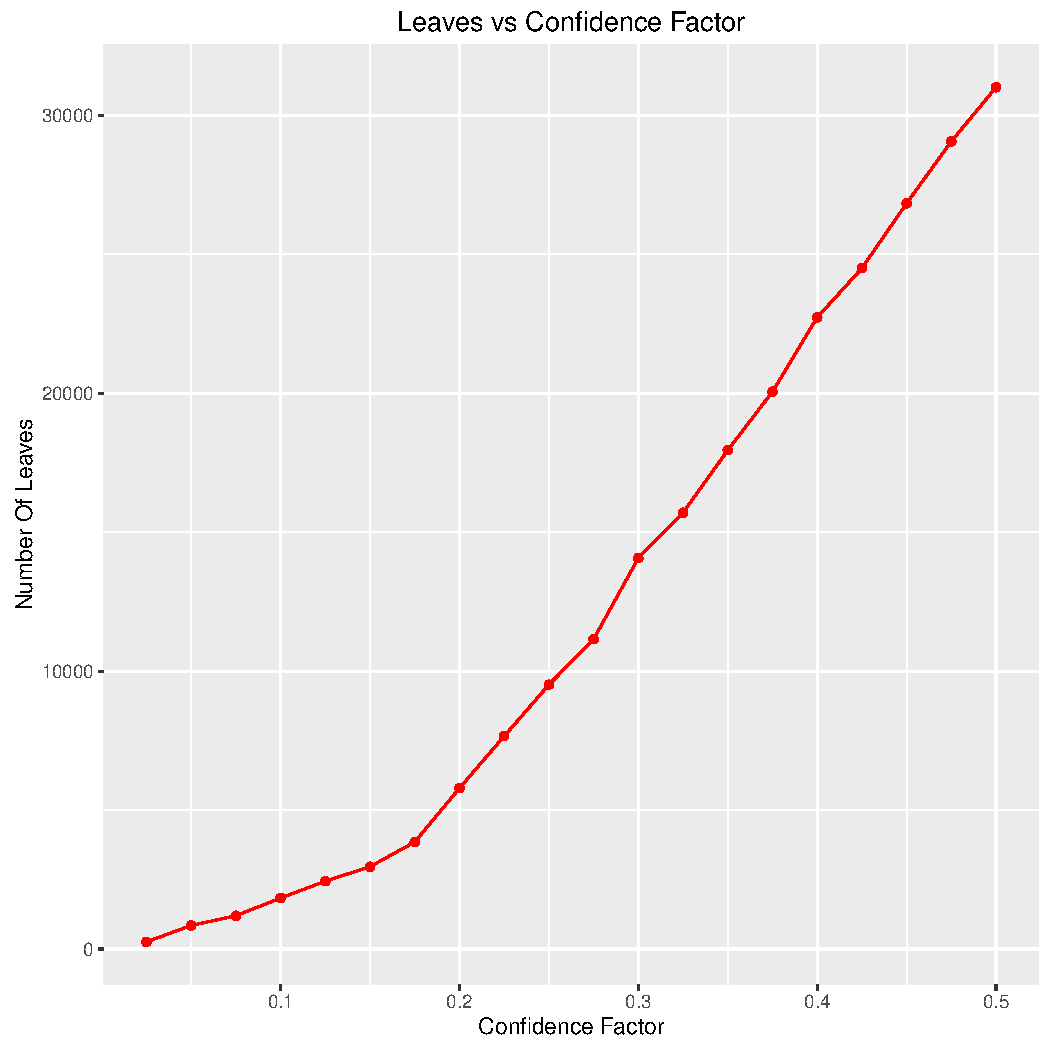
\includegraphics[width = 7cm]{3a.pdf}}
  \subfigure[Accuracy vs CF]{\label{b2}
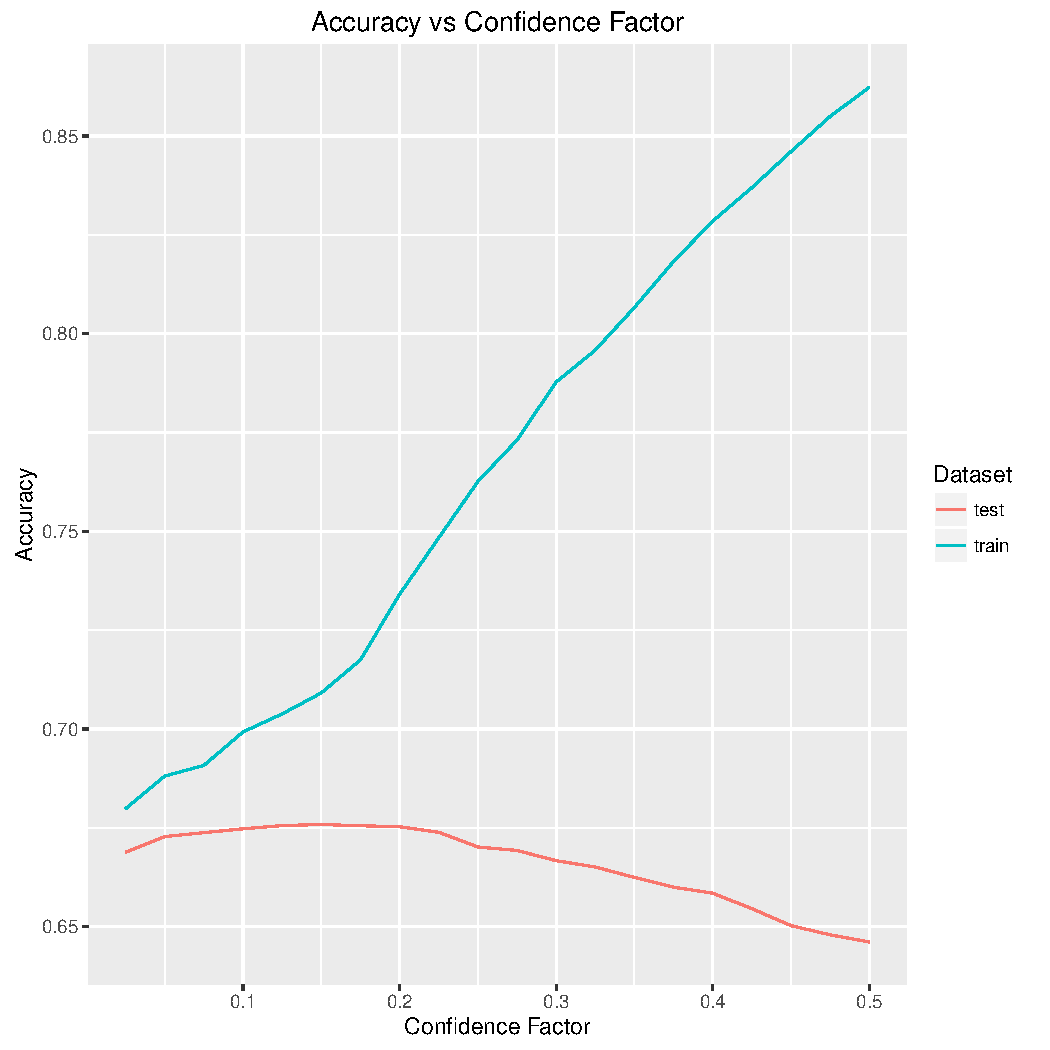
\includegraphics[width = 7cm]{3b.pdf}}
    \subfigure[ROC curve better tree]{\label{b3}
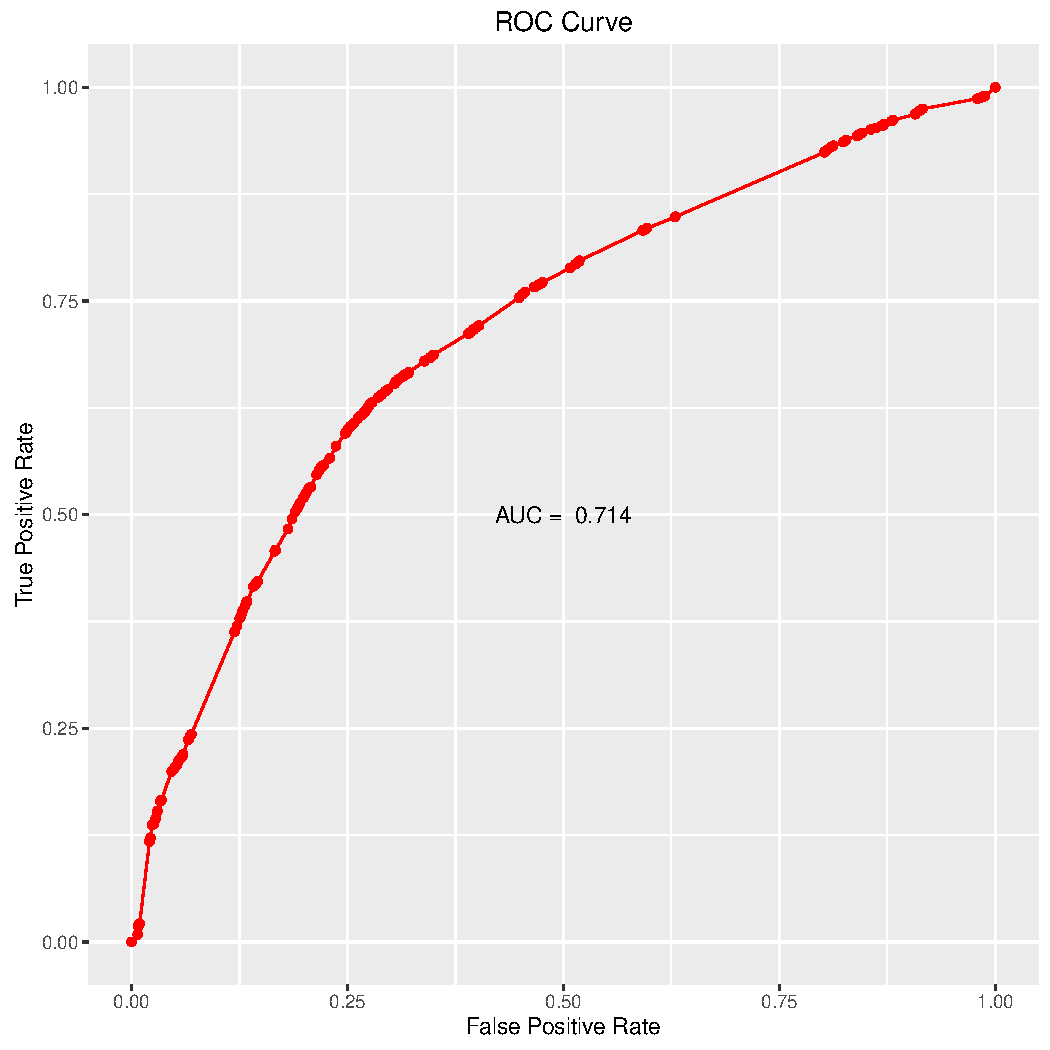
\includegraphics[width = 7cm]{3c.pdf}}
  \caption{overfitting and pruning}
  \label{fig:over}
\end{figure*}


\subsection{Tratamiento de datos faltantes}

\textbf{Descripción}: En la práctica, es común encontrarse y tener que trabajar con datasets que
contienen datos nulos o incompletos. Existen distintos métodos para tratar con ellos, en esta sección
se exploraron dos. Los cuales tratan de rellenar los datos faltantes con el valor modal del
atributo, y se diferencian en que uno toma en cuenta el valor de la clase para el individuo o registro
analizado, mientras que el otro no tiene en cuenta el valor de la clase.


\textbf{Metodología utilizada}:
Para el tratamiento de datos faltantes se indujo valores nulos al 80\% del dataset en los atributos con mayor GainRatio,
se preservó el 20\% de los datos para validación. A continuación se detallan las características de los atributos contemplados:

\definecolor{lightgray}{gray}{0.9}
\begin{table}[H]
\begin{center}
\caption{Atributos con mayor GainRatio}
\rowcolors{1}{}{lightgray}
\begin{tabular}{|>{\centering\arraybackslash}m{3cm}|>{\centering\arraybackslash}m{3cm}|}
\hline
  \rowcolor{blue!55} 
   \multicolumn{1}{|c|}{Atributo} &\multicolumn{1}{c|}{GainRatio} \\ \hline
    inst\_acreditada   &0.0436292021  \\ \hline
    estu\_metodo\_prgm &0.0295357038  \\ \hline
    \end{tabular}
\label{Gain Ratio}
\end{center}
\end{table}

El porcentaje de imputación de datos faltantes fue variando de 0 a 0.85 con incrementos de 0.025 generando
36 datasets con datos faltantes. 
En cada generación de datos faltantes, se relleno con la  moda los datos nulos del atributo inst\_acreditada  y con la modaclase para 
los valores nulos del atributo estu\_metodo\_prgm. Después se construyeron modelos con las estrategias
de relleno de datos faltantes anteriormente descritas variando el CF (Confidence Factor) de 0 a 0.5 y 
finalmente se evaluaron los mismos con el set de validación.

\textbf{Resultados esperados}: La performance sobre el set de validación no debería verse
sensiblemente afectada, al menos al introducir proporciones bajas o medias de datos faltantes, 
dada la robustez del algoritmo J48 para lidiar con esta problemática. 

Con respecto al tamaño del árbol, es de esperar que el mismo aumente
a medida que aumenta la función de poda y no por el porcentaje inducido de datos faltantes. 

\textbf{Análisis de los resultados}: En la figura~\ref{fig:missing}a,
se observa un patrón de comportamiento en las curvas de entrenamiento y validación para la accuracy,
dicho patron es similar a las curvas generadas en las corridas donde no se imputaron datos faltantes,
esto nos dice que el algoritmo J48 presenta resistencia y robustez a datos faltantes, 
ya que la performance se ve afectada más por la función de poda que por la imputación de datos faltantes.

En la figura~\ref{fig:missing}b, 
se observa claramente que el tamaño del árbol  incrementa debido al aumento de la función de poda 
(confidence factor), respecto al porcentaje de datos faltantes no se mira que este afecte en el tamaño del arbol.

En la figura~\ref{fig:missing}c, se observa un comportamiento similar
para los diferentes porcentajes de datos faltantes imputados,  la presición se comporta de igual forma manteniendo
la variación debido a la función de poda independientemente del porcentaje de datos faltantes.

Los anteriores supuestos los podemos confirmar claramente en la figura~\ref{fig:missing}d,
donde se puede mirar que a valores bajos CF hay un alto performance en el set de datos de validación, y a
medida que aumenta el valor de CF (eje x), también aumenta el valor de la performance del set de entrenamiento (tamaño
de la burbuja) así como baja la performance del set de testing (color de la burbuja) por este motivo el arbol se sobre ajusta
al conjunto de entrenamiento. 
Esta lectura es posible realizarla según el porcentaje de datos faltantes (de 0 a 0,85, en el eje Y; Cada serie de burbujas horizontales
corresponden al mismo experimento).

\textbf{Conclusión:} Los resultados se presentaron, en mayor o menor medida, en línea con lo esperado. La performance no 
se vio sensiblemente deteriorada al igual que el tamaño del árbol, aliniandose a los resultados esperados. 
Por tanto  el algoritmo de árboles J48 es robusto a datos faltantes,
ya que el rendimiento y  tamaño del árbol observados en los gráficos  se ven afectados por la función de poda y no por la
variación de datos faltantes.


\begin{figure*}
  \centering
  \subfigure[Accuracy vs CF]{\label{b1} 
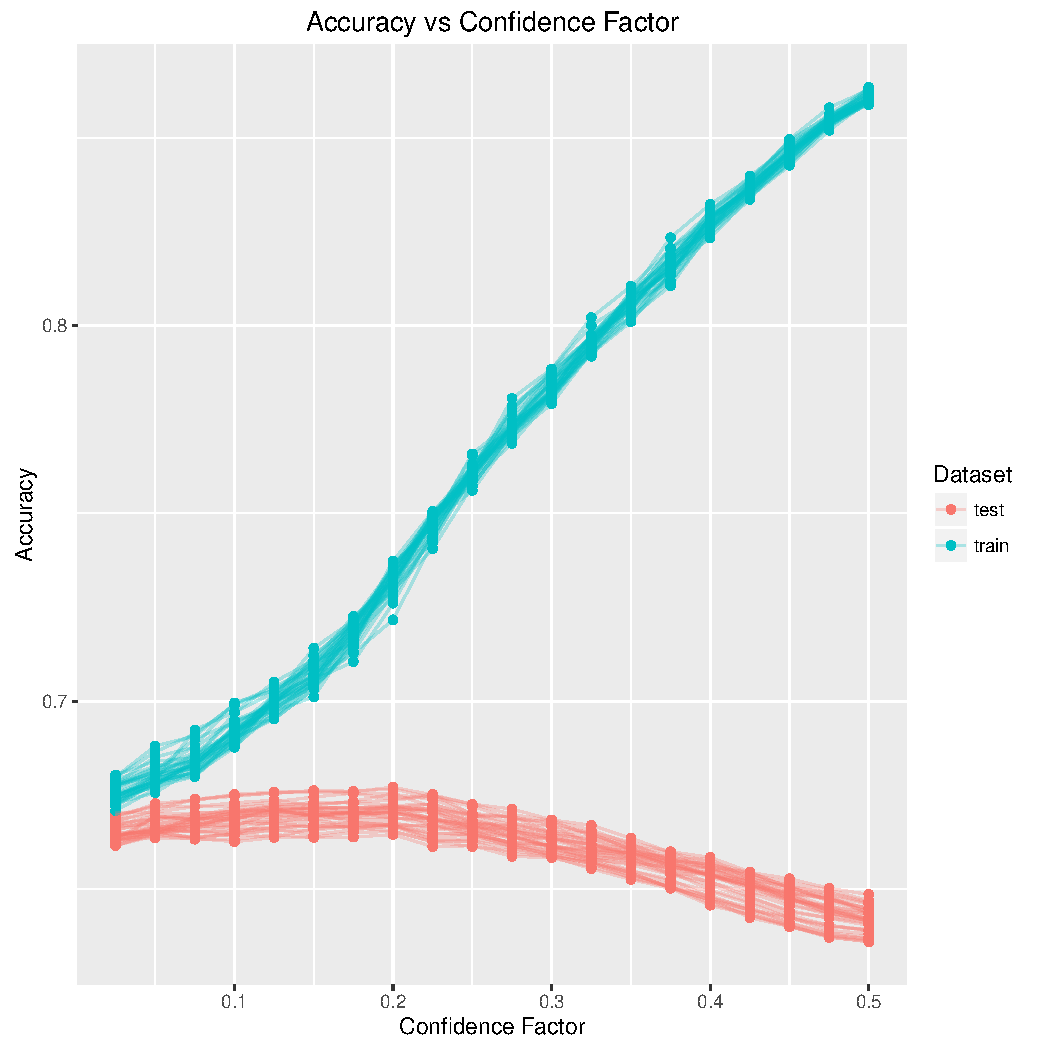
\includegraphics[width = 7cm]{4a.pdf}}
  \subfigure[Leaves vs missing percentage]{\label{b2} 
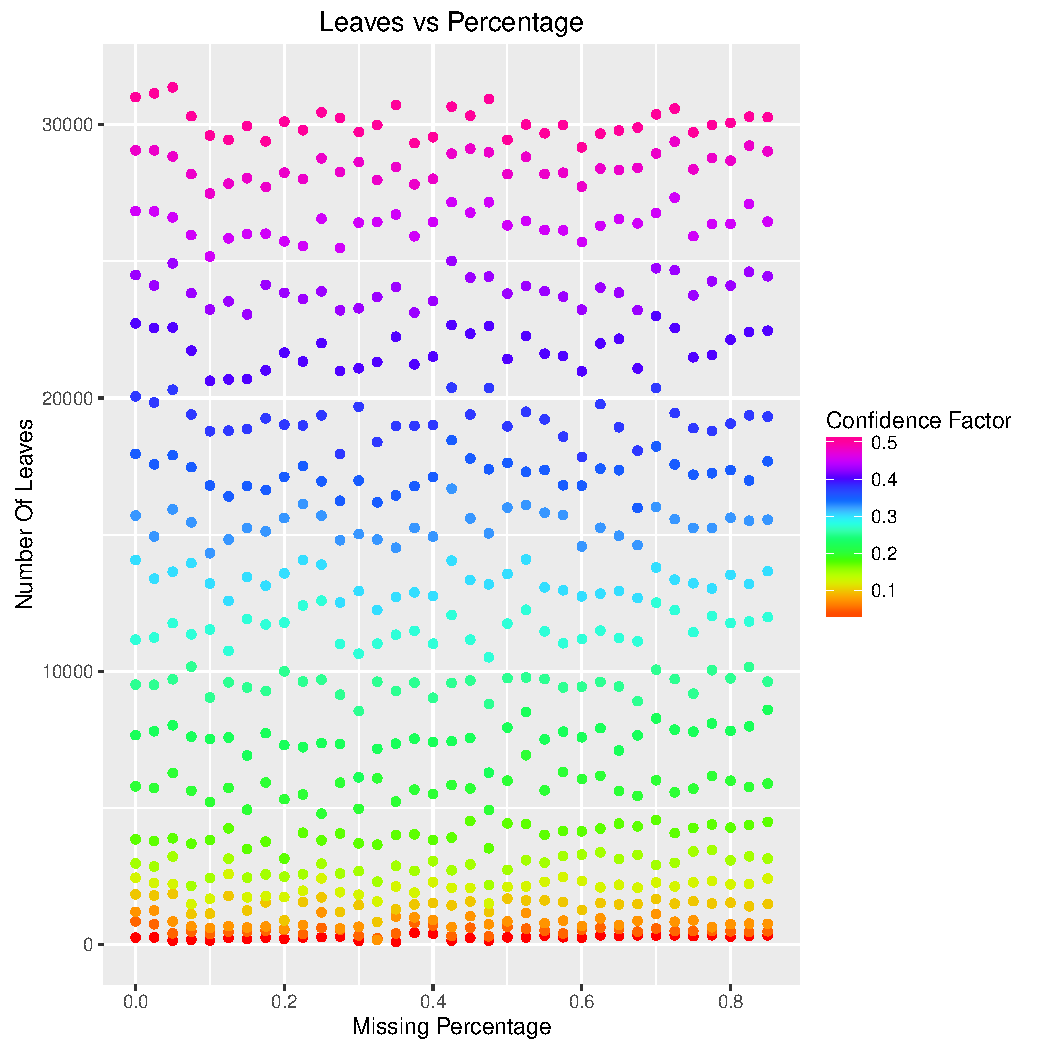
\includegraphics[width = 7cm]{4b.pdf}}
  \subfigure[Accuracy vs missing percentage]{\label{b3}
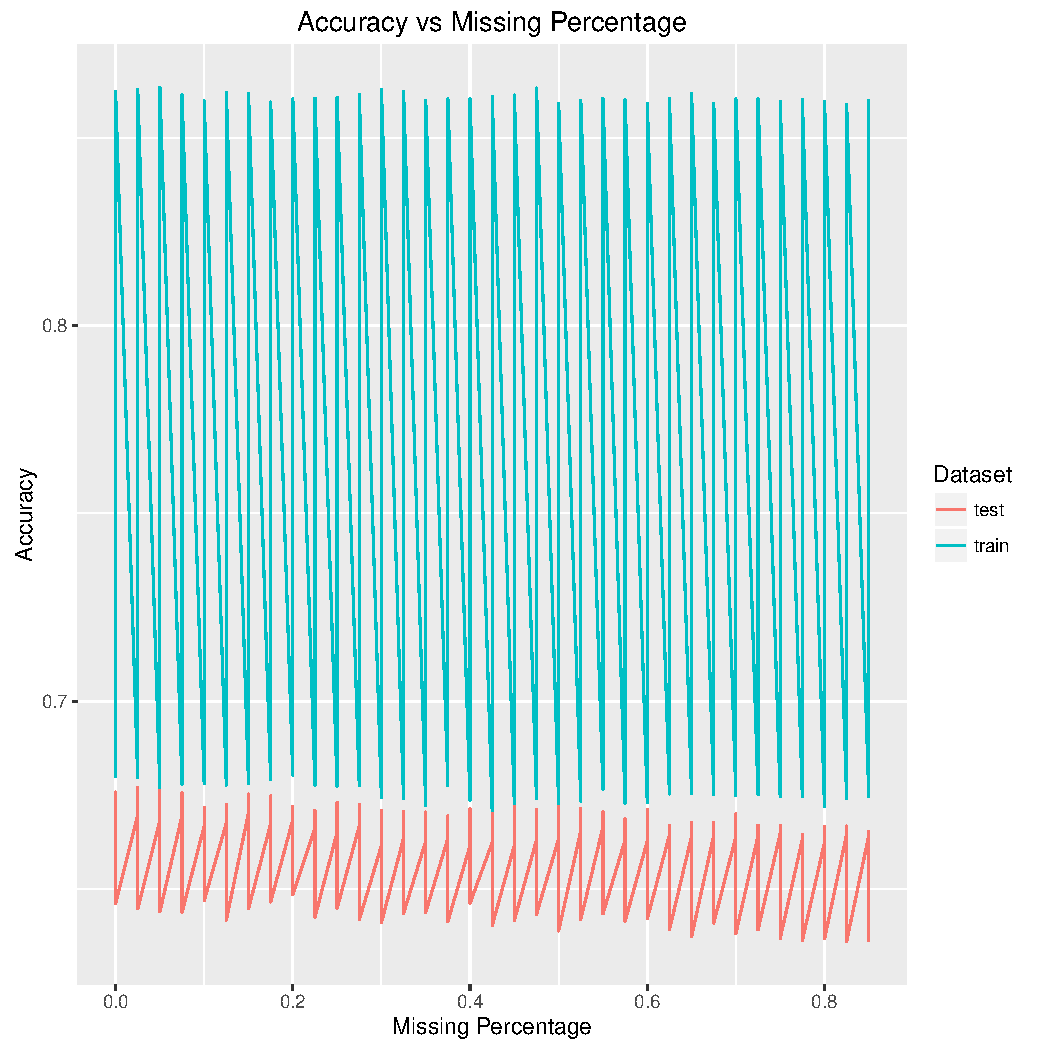
\includegraphics[width = 7cm]{4c.pdf}}
    \subfigure[Missing percentage vs CF]{\label{b4}
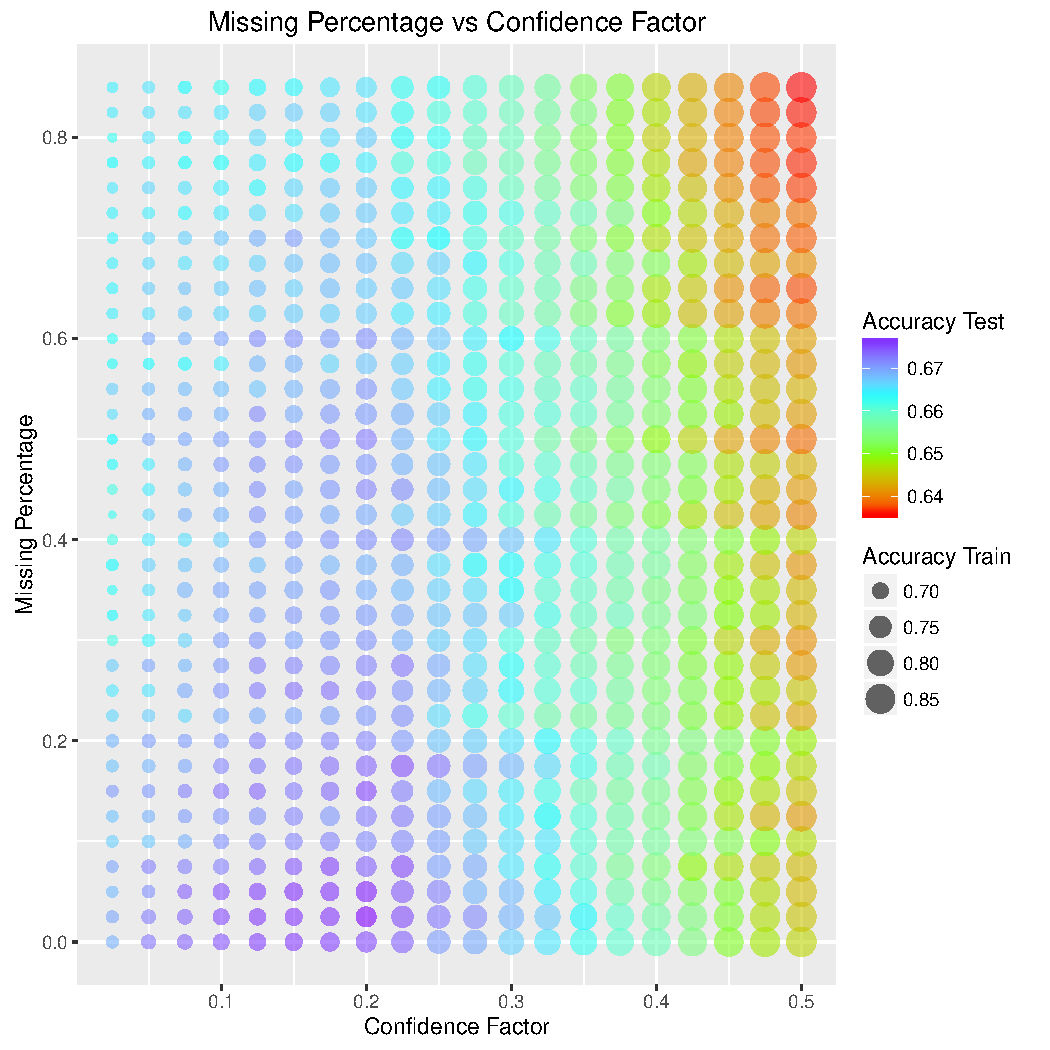
\includegraphics[width = 7cm]{4d.pdf}}
  \caption{Missing data}
  \label{fig:missing}
\end{figure*}

\subsection{Tratamiento de ruido}

En la figura~\ref{fig:5a} se muestra la grafica de la curva ROC para el mejor árbol,

\begin{figure}
  \centering
  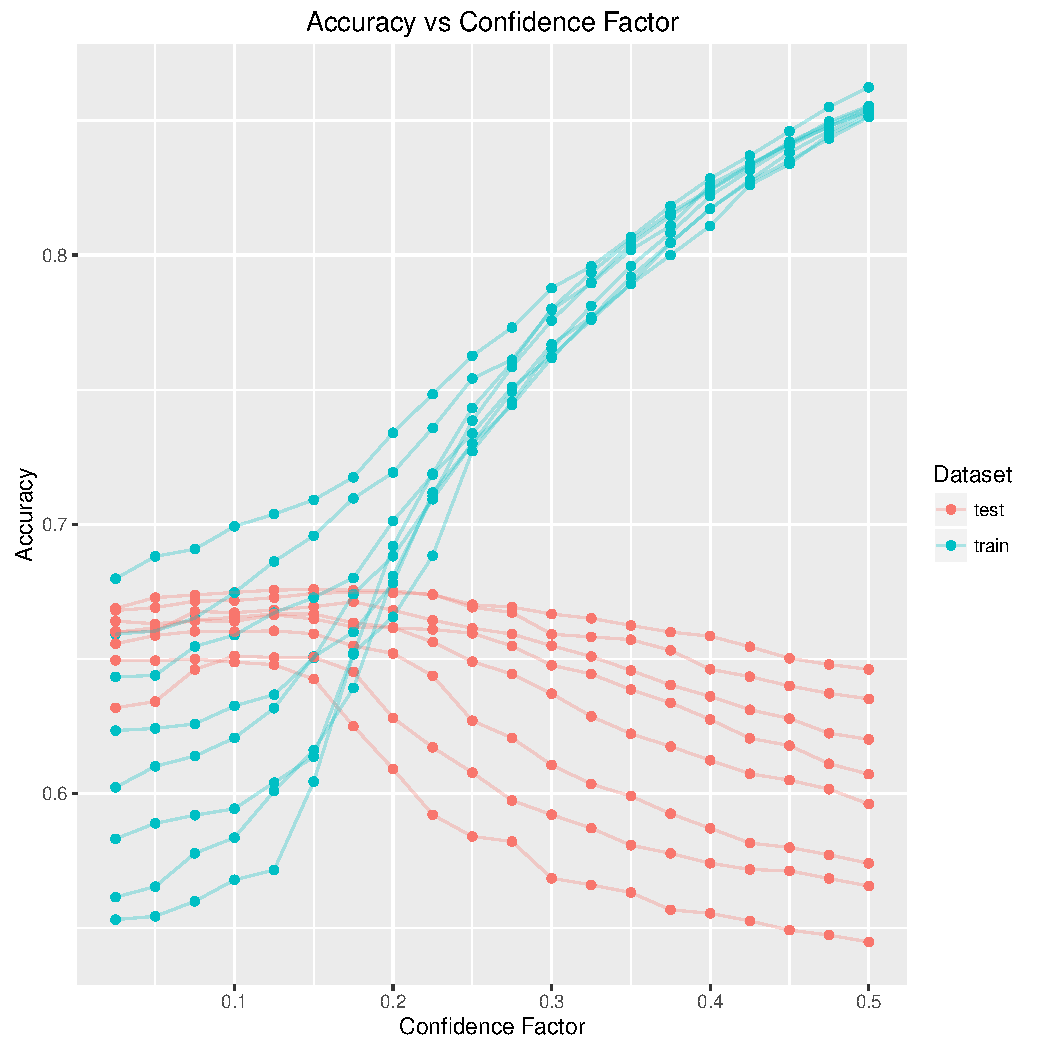
\includegraphics[width = 8cm]{5a.pdf}
  \caption{Accuracy vs CF with noise data}
  \label{fig:5a}
\end{figure}

En la figura~\ref{fig:5b} se muestra la grafica de la curva ROC para el mejor árbol,

\begin{figure}
  \centering
  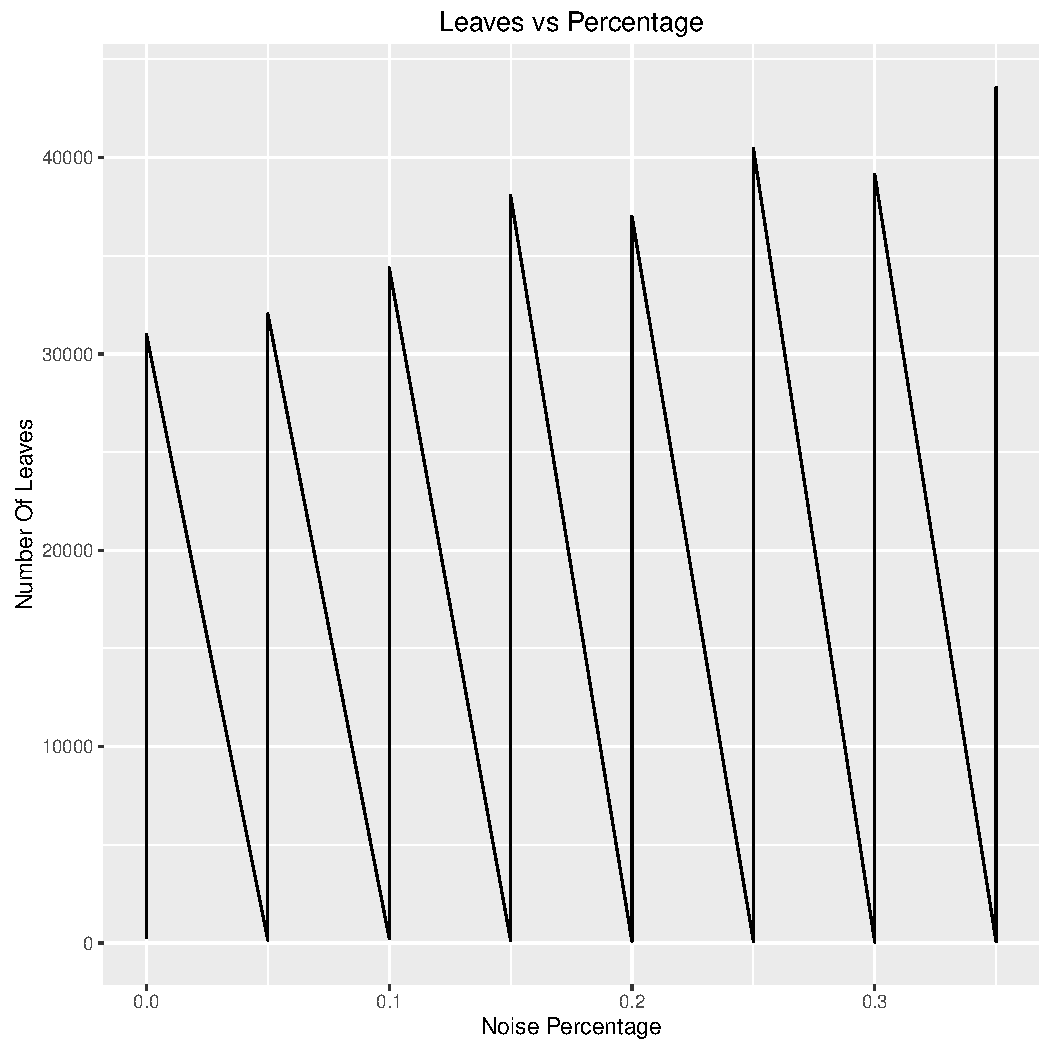
\includegraphics[width = 8cm]{5b.pdf}
  \caption{Leaves vs noice percentage}
  \label{fig:5b}
\end{figure}

En la figura~\ref{fig:5c} se muestra la grafica de la curva ROC para el mejor árbol,

\begin{figure}
  \centering
  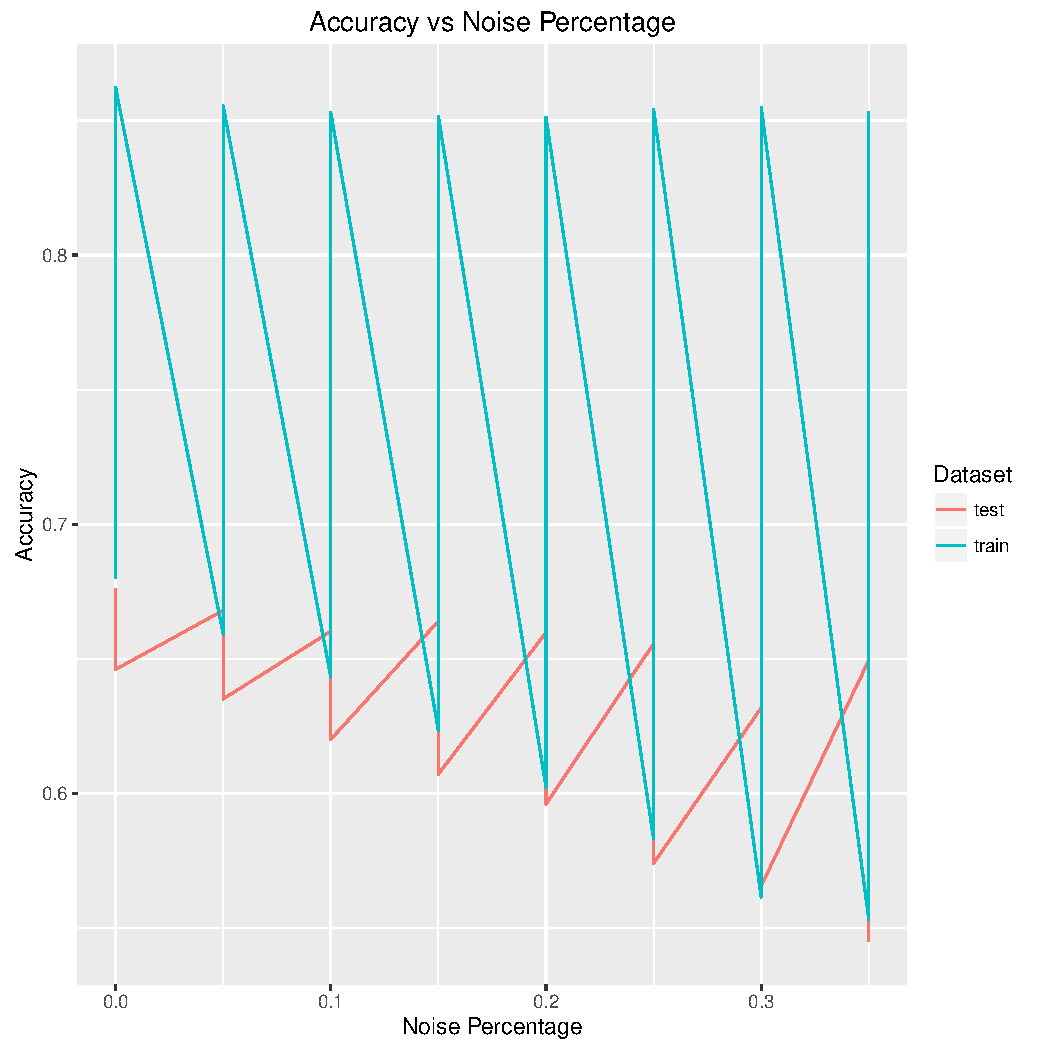
\includegraphics[width = 8cm]{5c.pdf}
  \caption{Accuracy vs noise percentage}
  \label{fig:5c}
\end{figure}

En la figura~\ref{fig:5d} se muestra la grafica de la curva ROC para el mejor árbol,

\begin{figure}
  \centering
  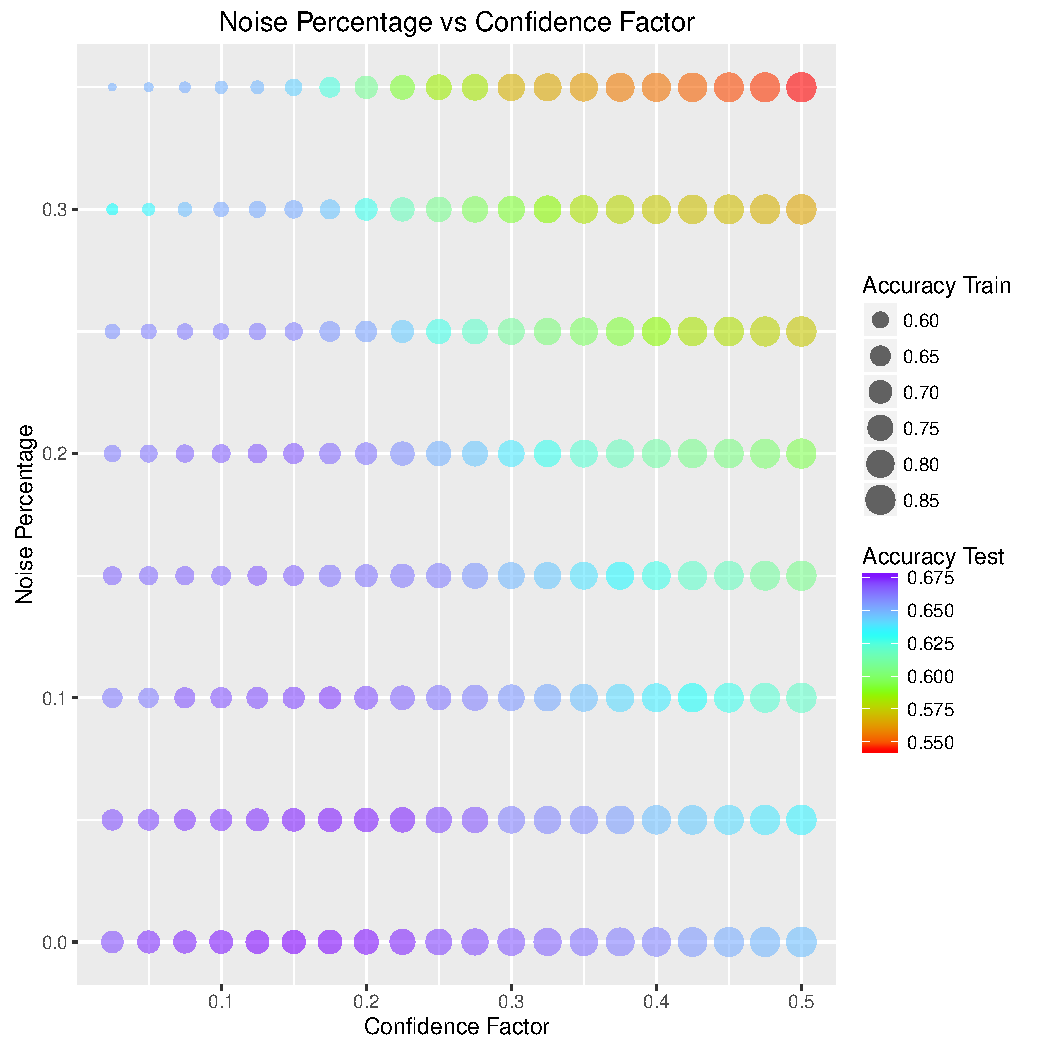
\includegraphics[width = 8cm]{5d.pdf}
  \caption{Noise percentage vs CF}
  \label{fig:5d}
\end{figure}


\subsection{Discretización}

En la figura~\ref{fig:6a} se muestra la grafica de la curva ROC para el mejor árbol,

\begin{figure}
  \centering
  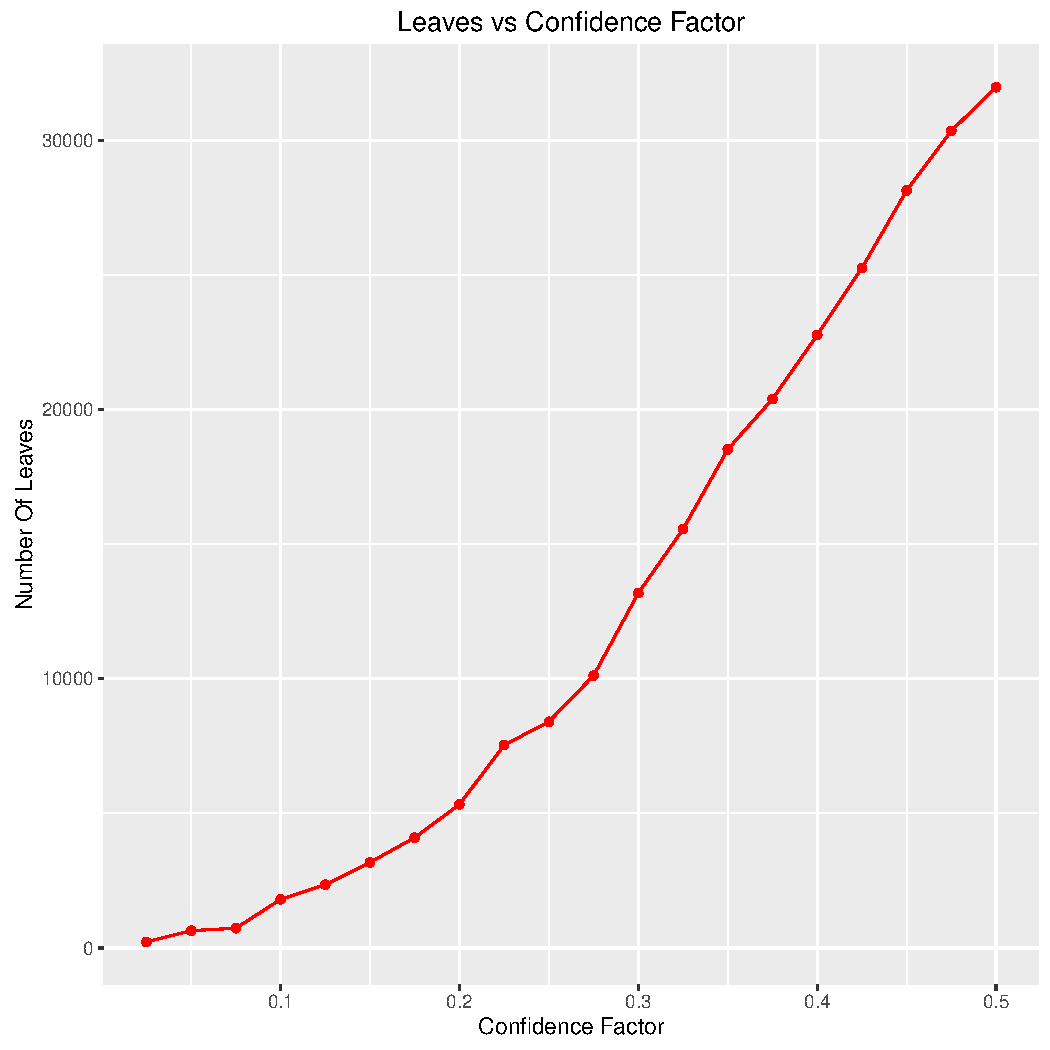
\includegraphics[width = 8cm]{6a.pdf}
  \caption{Number of leaves vs Confidence factor with supervised discretize}
  \label{fig:6a}
\end{figure}

En la figura~\ref{fig:6b} se muestra la grafica de la curva ROC para el mejor árbol,

\begin{figure}
  \centering
  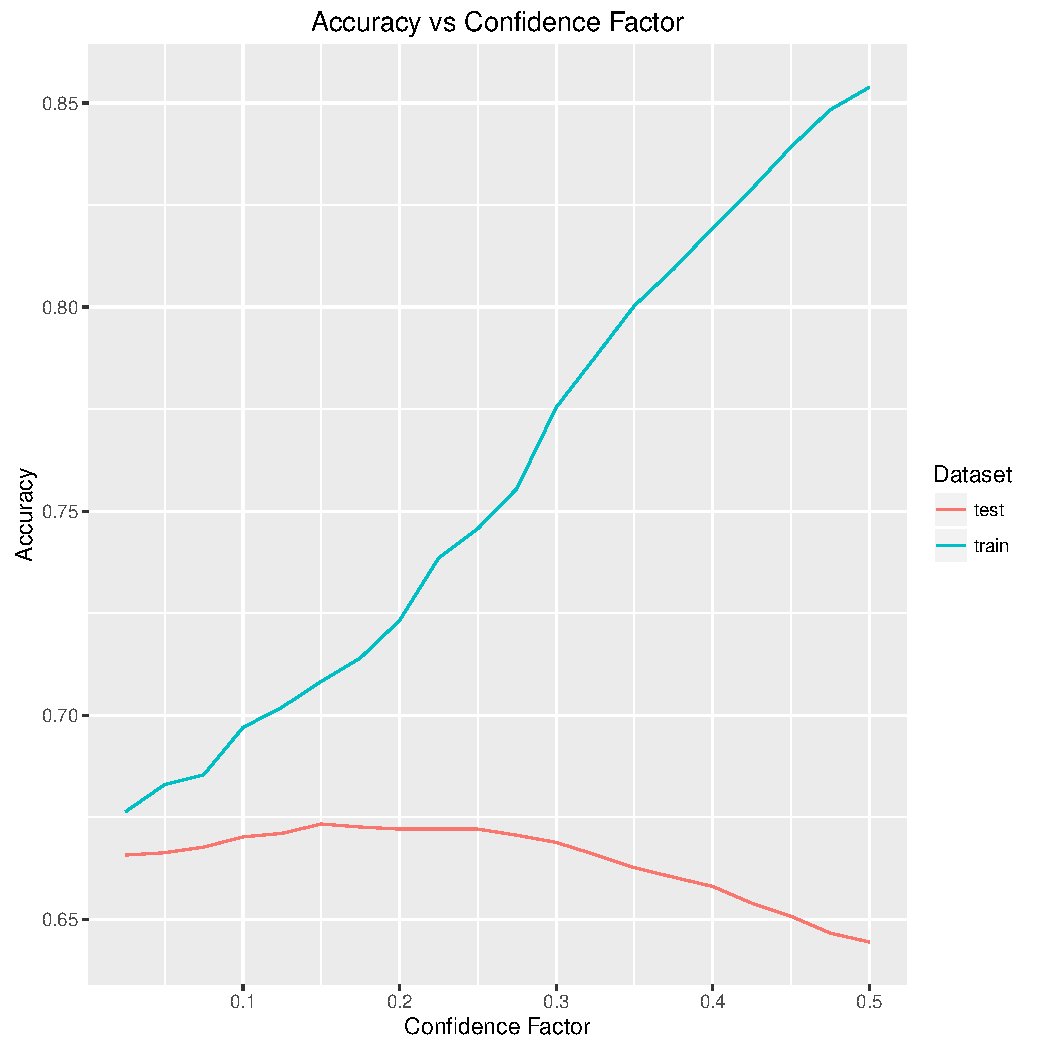
\includegraphics[width = 8cm]{6b.pdf}
  \caption{Accuracy vs Confidence factor with supervised discretized}
  \label{fig:6b}
\end{figure}

En la figura~\ref{fig:6c} se muestra la grafica de la curva ROC para el mejor árbol,

\begin{figure}
  \centering
  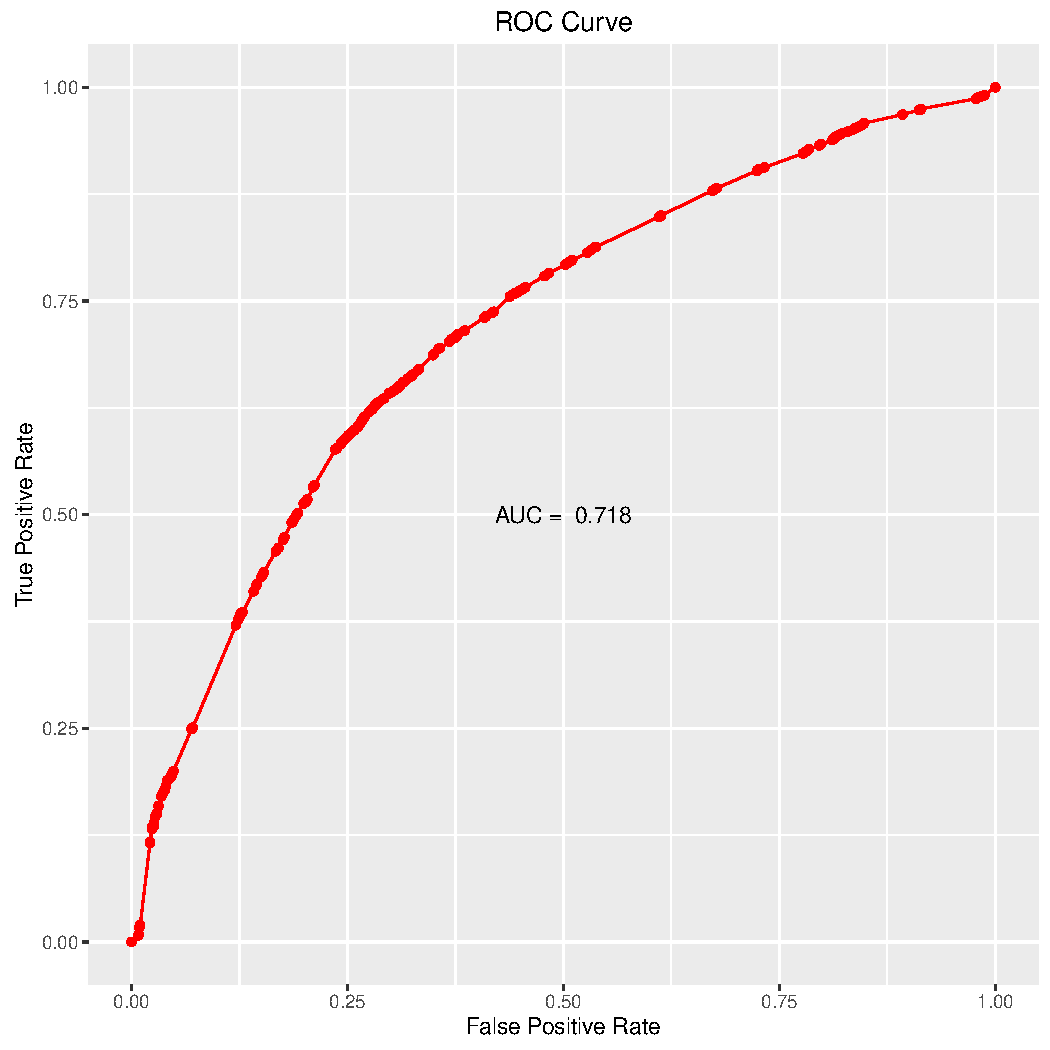
\includegraphics[width = 8cm]{6c.pdf}
  \caption{Curva ROC mejor árbol with supervised discretized}
  \label{fig:6c}
\end{figure}

En la figura~\ref{fig:6d} se muestra la grafica de la curva ROC para el mejor árbol,

\begin{figure}
  \centering
  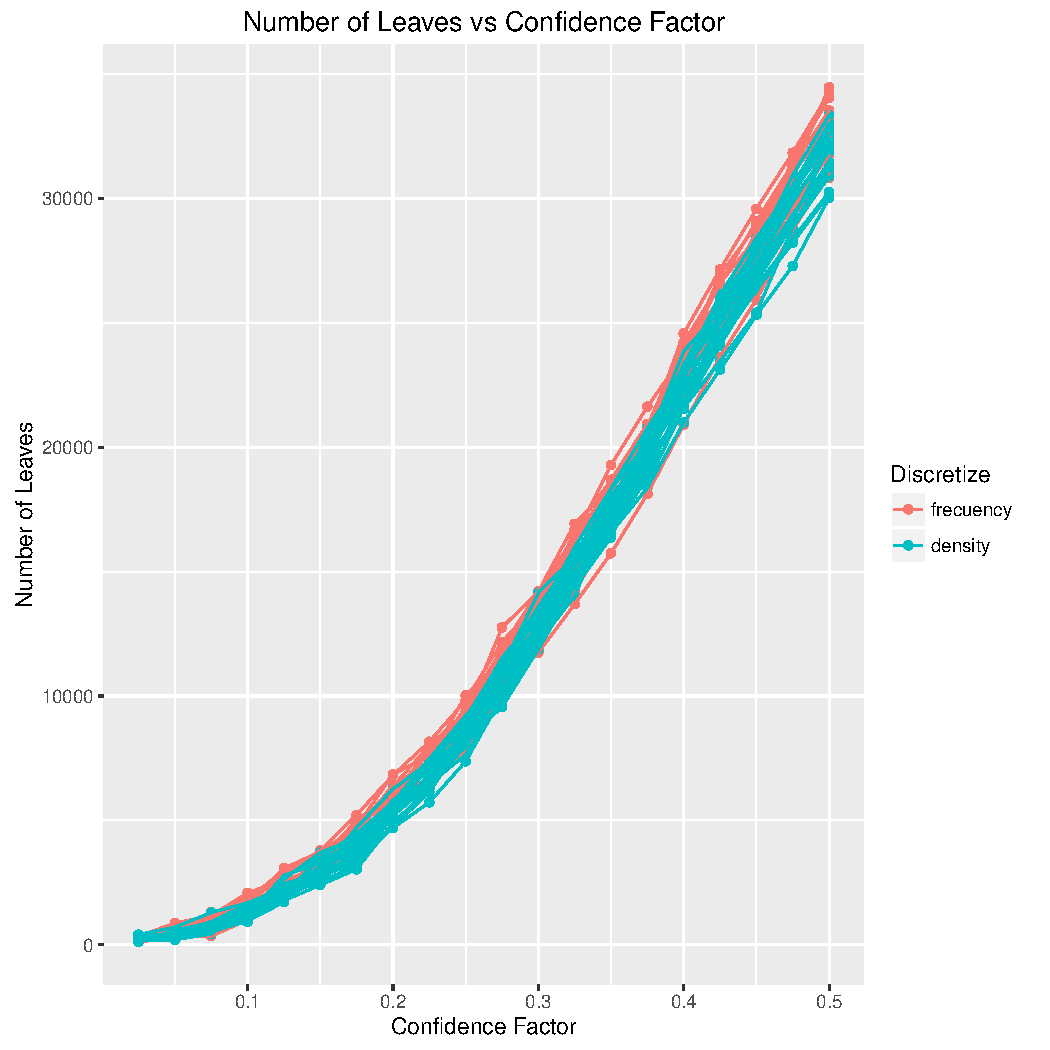
\includegraphics[width = 8cm]{6d.pdf}
  \caption{Leaves vs missing percentage with discretize}
  \label{fig:6d}
\end{figure}

En la figura~\ref{fig:6e} se muestra la grafica de la curva ROC para el mejor árbol,

\begin{figure}
  \centering
  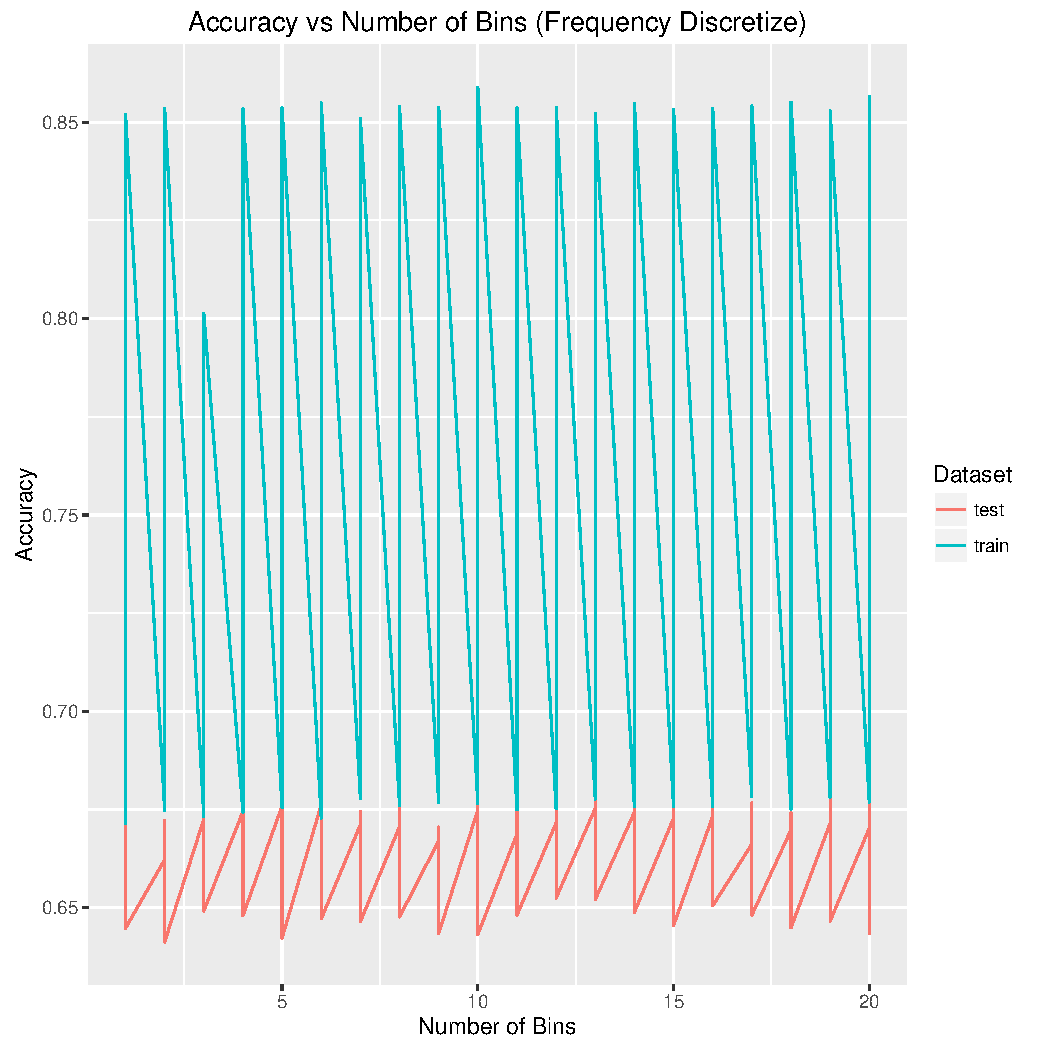
\includegraphics[width = 8cm]{6e.pdf}
  \caption{Accuracy vs Number of bins (Frequency discretize)}
  \label{fig:6e}
\end{figure}

En la figura~\ref{fig:6f} se muestra la grafica de la curva ROC para el mejor árbol,

\begin{figure}
  \centering
  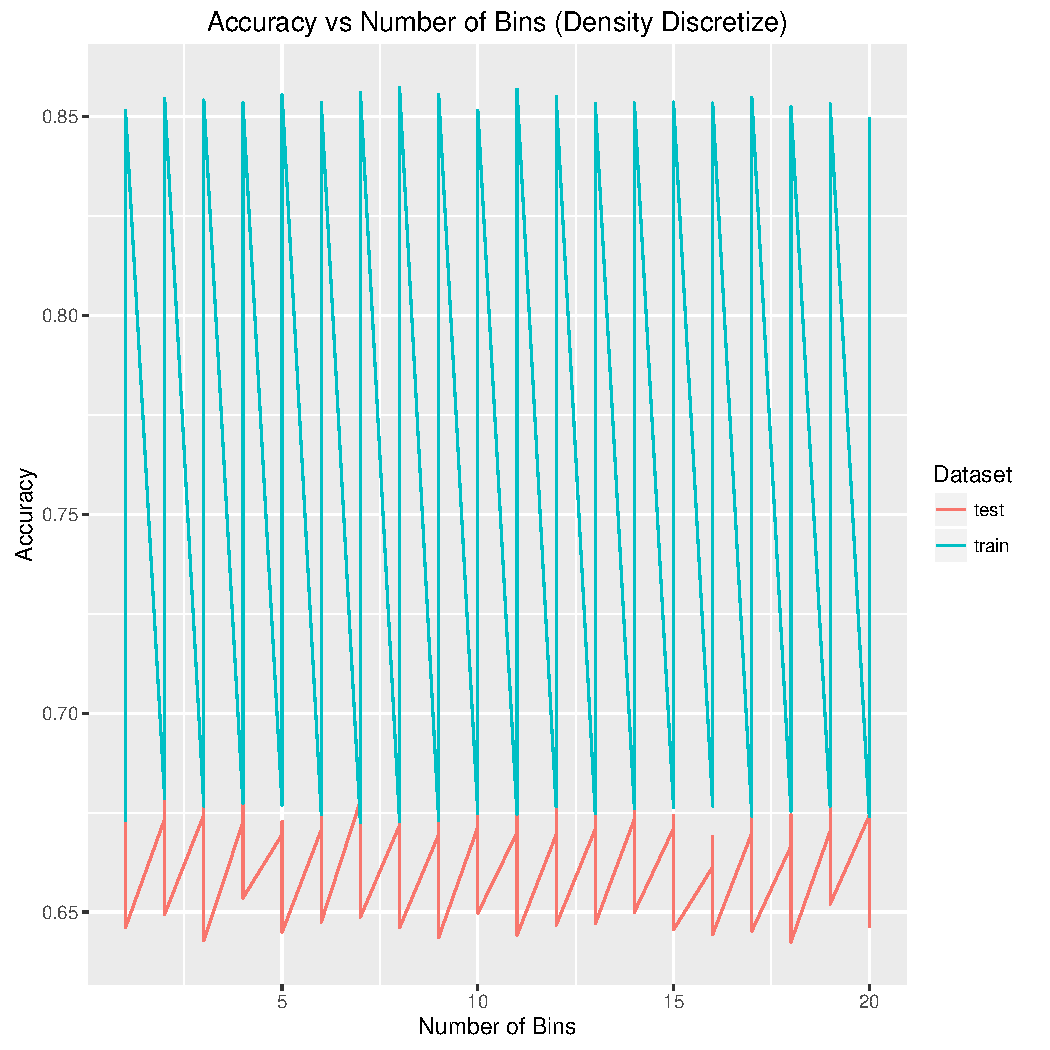
\includegraphics[width = 8cm]{6f.pdf}
  \caption{Accuracy vs Number of bins (Density discretize)}
  \label{fig:6f}
\end{figure}





\section{Conclusiones}

Para el conjunto de datos con el que se realizaron los diversos experimentos se concluye
que:

\begin{itemize}
 \item A nivel general, en los distintos experimentos el algoritmo de clasificación se
mostró robusto ante las distintas perturbaciones inducidas (datos faltantes, ruido,
discretización).

  \item Los valores de CF tienen una relación positiva con el tamaño del árbol medido en
cantidad de nodos, a mayores valores de CF el árbol es más grande. Asimismo
que al dejarse crecer el árbol la performance sobre el conjunto de entrenamiento
mejora, mientras que sobre el conjunto de validación mejora ligeramente hasta un
cierto punto (CF entre 15 y 18\%) y luego disminuye hasta mantenerse casi
constante. Todo esto pone de manifiesto la importancia que tiene la función de
poda para evitar el efecto de overfitting y la obtención de hipótesis cortas pero
robustas en relación al conjunto de validación.

  \item Al trabajar con datos faltantes, la performance sobre el set de validación no se vio
afectada de forma significativa, en especial a niveles medios / altos de CF (desde
25\% en adelante). Se observó una relación inversa entre el tamaño del árbol y el
porcentaje de faltantes. En cuanto a las estrategias de relleno, con modaclase los
resultados fueron notoriamente mejores a los de moda, consiguiendo incluso
niveles de clasificación por encima de los obtenidos al trabajar con el dataset
original. Este fenómeno podría ser objeto de un análisis más específico.

  \item Para bajos porcentajes ruido y podas severas, los efectos tanto sobre la cantidad
de nodos o tamaño de árbol y la performance en el conjunto de validación no
siguen una tendencia clara, manteniéndose en valores similares a los iniciales;
sin embargo para valores extremos tanto de ruido como de CF, se hace evidente
el incremento en la cantidad de nodos y la disminución de performance sobre el
conjunto de validación. Se puede decir que el árbol es robusto al ruido hasta un
cierto punto, el cual una vez superado tiende al fenómeno conocido como
overfitting.

  \item En cuanto al apartado de discretización, los resultados no fueron concluyentes.
Con las dos estrategias no supervisadas empleadas se obtuvieron resultados
similares en términos de tamaño del árbol y performance, imposibilitando elegir
una por sobre la otra. La discretización supervisada mostró ser la técnica
adecuada para niveles de CF superiores al 25\%, con un nivel de performance por
encima de la obtenida al trabajar con el dataset sin discretizar


\end{itemize}





%\appendices
%\section{Repositorio}
%El código fuente y conjunto de datos se encuentran en el repositorio de github.



% Can use something like this to put references on a page
% by themselves when using endfloat and the captionsoff option.
\ifCLASSOPTIONcaptionsoff
  \newpage
\fi


\bibliographystyle{IEEEtran}

\bibliography{IEEEabrv,bibliography}



\end{document}
